\documentclass[a4paper, DIV12, headsepline]{scrartcl}

% common packages
\usepackage{lmodern}
\usepackage[T1]{fontenc}
\usepackage[utf8]{inputenc}
\usepackage[english]{babel}
\usepackage{amsfonts}
\usepackage{amssymb}
\usepackage{amsmath}
\usepackage{siunitx}
\usepackage{graphicx}
\usepackage{url}
\usepackage{listings}
\usepackage{tikz}
\usepackage{enumitem}
\usepackage[labelfont=bf]{caption}

% set head and foot
\usepackage{scrpage2}
\pagestyle{scrheadings}
\clearscrheadfoot
\ihead{Lab 3 -- Report}
\ohead{Group 25: Hui Jing (cid: huij), Tobias Fuchs (cid: fuchs)}
\cfoot{\pagemark}

% set pdf options
\usepackage[pdfborder={0 0 0}, bookmarksopen=true, bookmarksnumbered=true, pdftitle={Lab 3 Report}, pdfauthor={Hui Jing, Tobias Fuchs}, pdfsubject={Report}]{hyperref}

\begin{document}

\section*{Report for Lab 3}
\subsection*{Task 1 -- ERT}
\begin{enumerate}[label=\alph*)]
\item 3 levels of cache is available in the machine.

 \texttt{lscpu |grep -i cache}
\begin{verbatim}
L1d cache:           32K
L1i cache:           32K
L2 cache:            256K
L3 cache:            6144K
\end{verbatim}
% L1: 64KiB (32KiB Instruction-Cache, 32KiB Data-Cache), L2: 256KiB, L3: 6144KiB = 6 MiB 

\item
Memory Bandwith: L1: \SI{441.2}{GiB/s}, L2: \SI{55.81}{GiB/s}, L3: \SI{41.94}{GiB/s}, DRAM: \SI{31.21}{GiB/s}

Machine Performance: \SI{64.8} {GFLOPs/sec}
\end{enumerate}

\subsection*{Task 2 -- Calculating AI using SDE}
\begin{enumerate}[label=\alph*)]
\item According to the \textsc{Intel Sde} tool, the total number of \textsc{Flops} for different numbers of threads and problem sizes is given in Table~\ref{tab:tab1}.
\begin{table}[htbp]
\centering
\begin{tabular}{cSSSS}
\hline
 & \multicolumn{4}{c}{Problem Sizes} \\
Threads & \SI{0.5}{M} & \SI{1}{M} & \SI{10}{M} & \SI{100}{M} \\
\hline
1 & \SI{9000942}{FLOP} & \SI{18000974}{FLOP} & \SI{180000950}{FLOP} & \SI{1800000934}{FLOP} \\
2 & \SI{9000926}{FLOP} & \SI{18000974}{FLOP} & \SI{180000918}{FLOP} & \SI{1800000914}{FLOP} \\
4 & \SI{9000906}{FLOP} & \SI{18000942}{FLOP} & \SI{180000926}{FLOP} & \SI{1800000918}{FLOP} \\
\hline
\end{tabular}
\caption{FLOP numbers for different configurations.}
\label{tab:tab1}
\end{table}


\item Furthermore, the total number of bytes (read and write) is given in Table~\ref{tab:tab2}.
\begin{table}[htbp]
\centering
\begin{tabular}{cSSSS}
\hline
 & \multicolumn{4}{c}{Problem Sizes} \\
Threads & \SI{0.5}{M} & \SI{1}{M} & \SI{10}{M} & \SI{100}{M} \\
\hline
1 & \SI{120896483}{B} & \SI{240897640}{B} & \SI{2400901149}{B} & \SI{24000894174}{B} \\
2 & \SI{126182868}{B} & \SI{246130313}{B} & \SI{2408254332}{B} & \SI{24012186264}{B} \\
4 & \SI{145309375}{B} & \SI{260864133}{B} & \SI{2426388194}{B} & \SI{24034106726}{B} \\
\hline
\end{tabular}
\caption{Number of Bytes for different configurations.}
\label{tab:tab2}
\end{table}

\item According to the \textsc{Intel Sde} tool, the running times of the \texttt{stream} benchmark for different configurations is given in Table~\ref{tab:tab3}.
\begin{table}[htbp]
\centering
\begin{tabular}{cSSSS}
\hline
 & \multicolumn{4}{c}{Problem Sizes} \\
Threads & \SI{0.5}{M} & \SI{1}{M} & \SI{10}{M} & \SI{100}{M} \\
\hline
1 & \SI{0.051645}{s} & \SI{0.101378}{s} & \SI{0.878443}{s} & \SI{8.699119}{s} \\
2 & \SI{0.040350}{s} & \SI{0.060514}{s} & \SI{0.467490}{s} & \SI{4.452410}{s} \\
4 & \SI{0.045516}{s} & \SI{0.057817}{s} & \SI{0.275754}{s} & \SI{2.329622}{s} \\
\hline
\end{tabular}
\caption{Running times for different configurations.}
\label{tab:tab3}
\end{table}

\item The arithmetic intensity (AI) can then calculated by
\begin{equation}
\operatorname{AI} = \frac{\operatorname{FLOP}}{\operatorname{Bytes}} \enspace \textrm{.}
\end{equation}
The arithmetic intensities for different configurations are given in Table~\ref{tab:tab4}.
\begin{table}[htbp]
\centering
\begin{tabular}{cSSSS}
\hline
 & \multicolumn{4}{c}{Problem Sizes} \\
Threads & \SI{0.5}{M} & \SI{1}{M} & \SI{10}{M} & \SI{100}{M} \\
\hline
1 & \SI{0.074451}{FLOP/B} & \SI{0.074724}{FLOP/B} & \SI{0.074972}{FLOP/B} & \SI{0.074997}{FLOP/B} \\
2 & \SI{0.071332}{FLOP/B} & \SI{0.073136}{FLOP/B} & \SI{0.074743}{FLOP/B} & \SI{0.074962}{FLOP/B} \\
4 & \SI{0.061943}{FLOP/B} & \SI{0.069005}{FLOP/B} & \SI{0.074185}{FLOP/B} & \SI{0.0748936}{FLOP/B} \\
\hline
\end{tabular}
\caption{Arithmetic Intensities for different configurations.}
\label{tab:tab4}
\end{table}

\item The performance is then
\begin{equation}
\operatorname{Perf} = \frac{\operatorname{FLOP}}{\operatorname{s}} \enspace \textrm{.}
\end{equation}
The performances for different configurations are given Table~\ref{tab:tab5}.
\end{enumerate}
\begin{table}[htbp]
\centering
\begin{tabular}{cSSSS}
\hline
 & \multicolumn{4}{c}{Problem Sizes} \\
Threads & \SI{0.5}{M} & \SI{1}{M} & \SI{10}{M} & \SI{100}{M} \\
\hline
1 & \SI{0.174285}{GFLOP/s} & \SI{0.177563}{GFLOP/s} & \SI{0.204909}{GFLOP/s} & \SI{0.206918}{GFLOP/s} \\
2 & \SI{0.223071}{GFLOP/s} & \SI{0.297468}{GFLOP/s} & \SI{0.385037}{GFLOP/s} & \SI{0.404276}{GFLOP/s} \\
4 & \SI{0.197753}{GFLOP/s} & \SI{0.311343}{GFLOP/s} & \SI{0.652759}{GFLOP/s} & \SI{0.772658}{GFLOP/s} \\
\hline
\end{tabular}
\caption{Performances for different configurations.}
\label{tab:tab5}
\end{table}

\subsection*{Task 3 -- Performance Analysis Results}
\begin{enumerate}[label=\alph*)]
\item The figure below shows the roofline model and the obtained measurements. We observed that the GFLOP/s increased with an increasing number of threads and also increased with an increasing size of the stream file.  The GFLOP/s obtained shows the application is memory bound, however, it did not reach the maximum performance, i.e. the algorithm can still be improved.
\begin{center}
	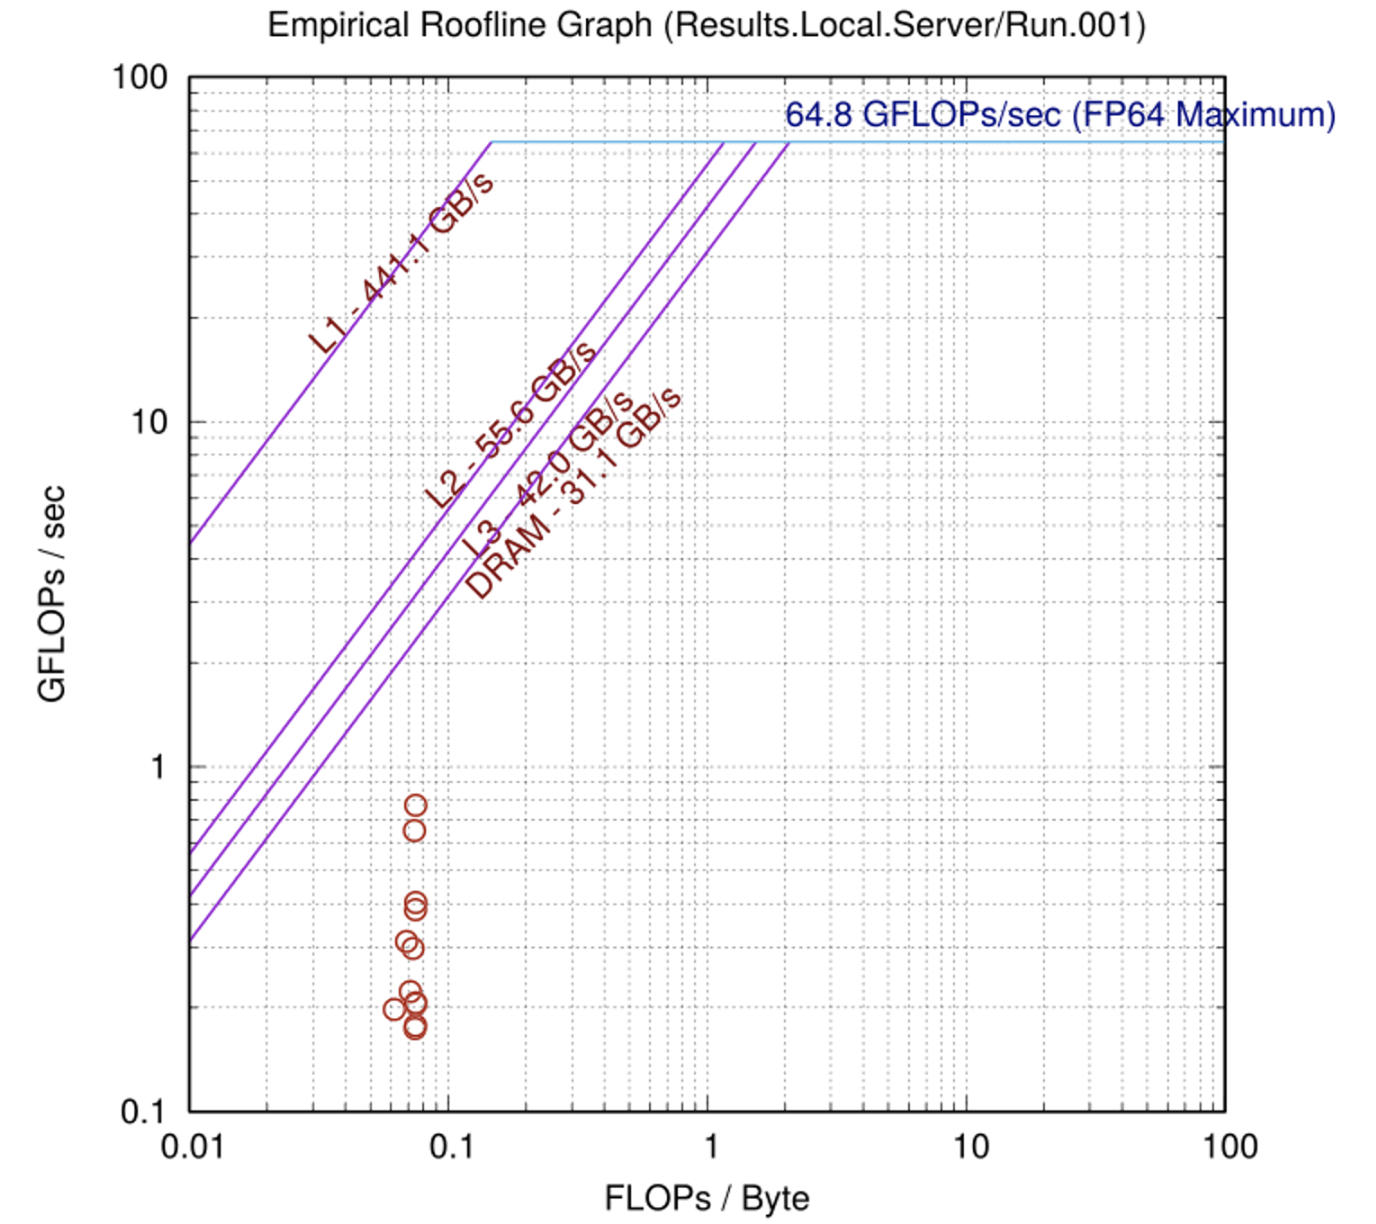
\includegraphics[scale=0.5]{roofline_graph}
\end{center}
% - Attainable Flop/s = min(peak Flop/s, AI * peak GB/s)
% - Memory Bandwidth from Task 1
% - One diagram for each memory type
% - Results in excel file code/lab3/lab3.xlsx
\end{enumerate}

\end{document}
